Der Begriff REST API steht für "Representational State Transfer - Application Programm Interface" und ermöglicht den Austausch von Informationen, welche sich auf unterschiedlichen Systemen befinden. In diesem Kapitel wird es vorrangig, um die von diesem Team entwickelten Endpunkte des Backends gehen. Grundsätzlich wird in unserer Arbeit zwischen zwei großen, übergeordneten Endpunkten (User und Projekte) unterschieden, bei welchem man anschließend das dazugehörige JSON-Objekt zurück geliefert bekommt. Mit den Übergabeparametern wird im Router-File entschieden, welche Datenbankabfrage gerade aus dem Frontend aufgerufen wurde. Dazu wird der Parameter im Frontend, mit Aufruf der Seite, in die URL eingebaut und anschließend an das Backend weitergeleitet, wo schlussendlich entschieden wird, welche Funktion aufgerufen werden muss.
\newline
Im oben gezeigten Beispiel ist ausgeführt, wie diese Überprüfung im spezifischen Fall des Users aussieht. Zu Beginn wird überprüft, ob der gewünschte Parameter übermittelt wurde, wenn dieser vorhanden ist, wird er mit allen Möglichkeiten verglichen und im Falle eines Treffers die Handler-Funktion aufgerufen, in welchem sich die tatsächliche Datenbankabfrage befindet. Alle implementierten Optionen, wurden im Vorfeld von dieser Diplomarbeit von der Partnerfirma erarbeitet und im Zuge des Praktikums, vom Projektteam eingearbeitet.
\newline
\begin{figure}
    \centering
    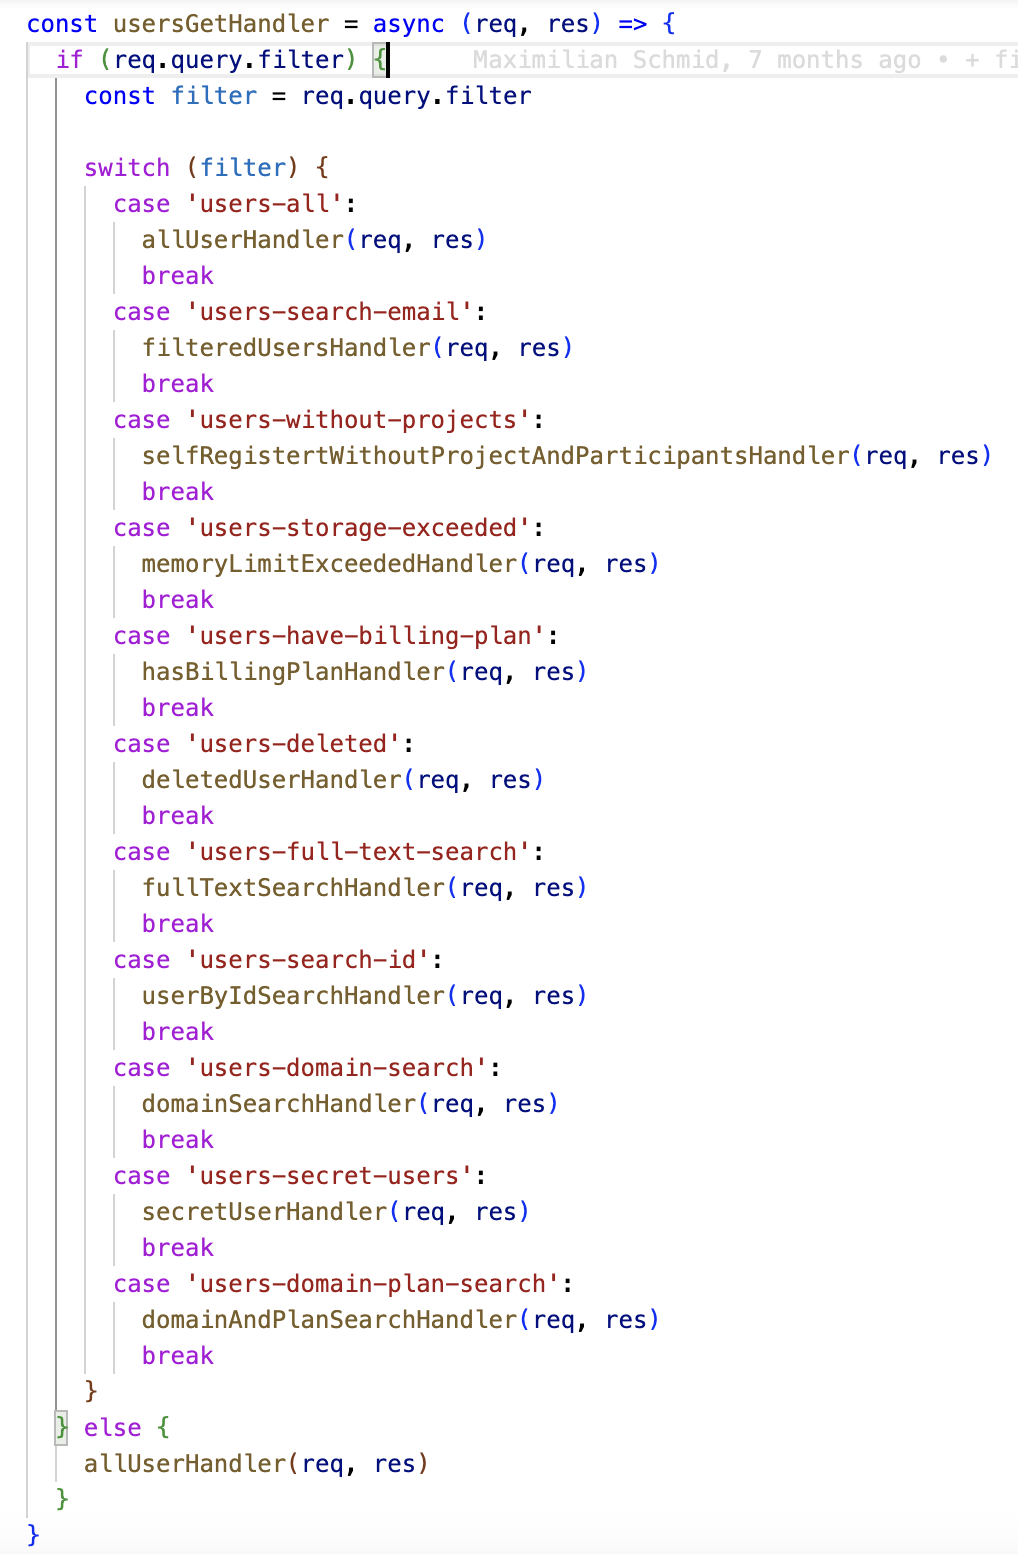
\includegraphics[width=0.4\linewidth]{pics/REST_API_Img.png}
    \caption{User-GET-Handler}
    \label{fig:enter-label}
\end{figure}